\chapter[图的撰写规范]{图的撰写规范{\song\xiaosi \textcolor{red}{(黑体小二号加粗,段后1行,居中)}}}
\label{cha:command}


\section[二级标题]{二级标题{\song\xiaosi \textcolor{red}{(黑体小三号字加粗,前后段间距0.5行,不空格)}}}
正文段落格式为:宋体/Times New Roman 小四号字,1.25倍行距,首行缩进2字符

\subsection[三级标题]{三级标题{\song\xiaosi \textcolor{red}{(黑体四号字加粗,前后段间距0.25行,不空格)}}}
要精选、简明,切忌与表及文字表述重复。

要清楚,但坐标比例不要过份放大,同一图上不同曲线的点要分别用不同形状标出。

图中的术语、符号、单位等应同文字表述一致。

图按章编号,图序及图名置于图的下方,宋体五号字加粗,居中。

若图有附注,采用英文小写字母顺序编号,附注写在图的下方。 

图与正文之间要有一行的间距,如:

单图
\begin{figure}[!htbp]
    \centering
    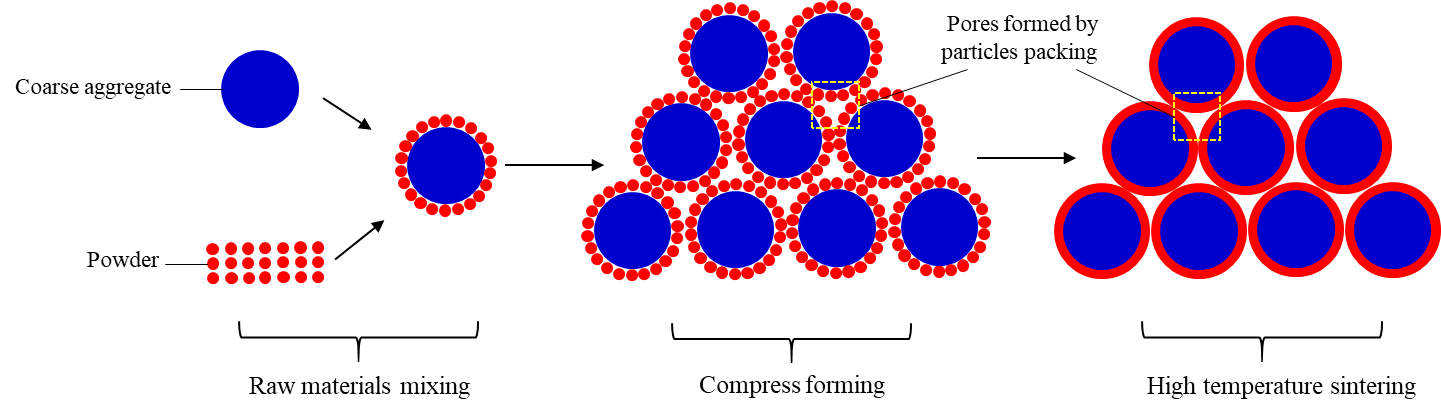
\includegraphics[width=1.0\textwidth]{Fig3-1.png}
    \bicaption{颗粒堆积型多孔材料制备过程和结构示意图}
    {Schematic diagram of the preparation process and structure of porous permeable brick generated by particle packing\\
    \textcolor{red}{(宋体、Times New Roman 5号字加粗,居中置于图的下方)}}
    \label{Fig3-1}
\end{figure}
\clearpage
多图
\begin{figure}[!htbp]
    \centering
    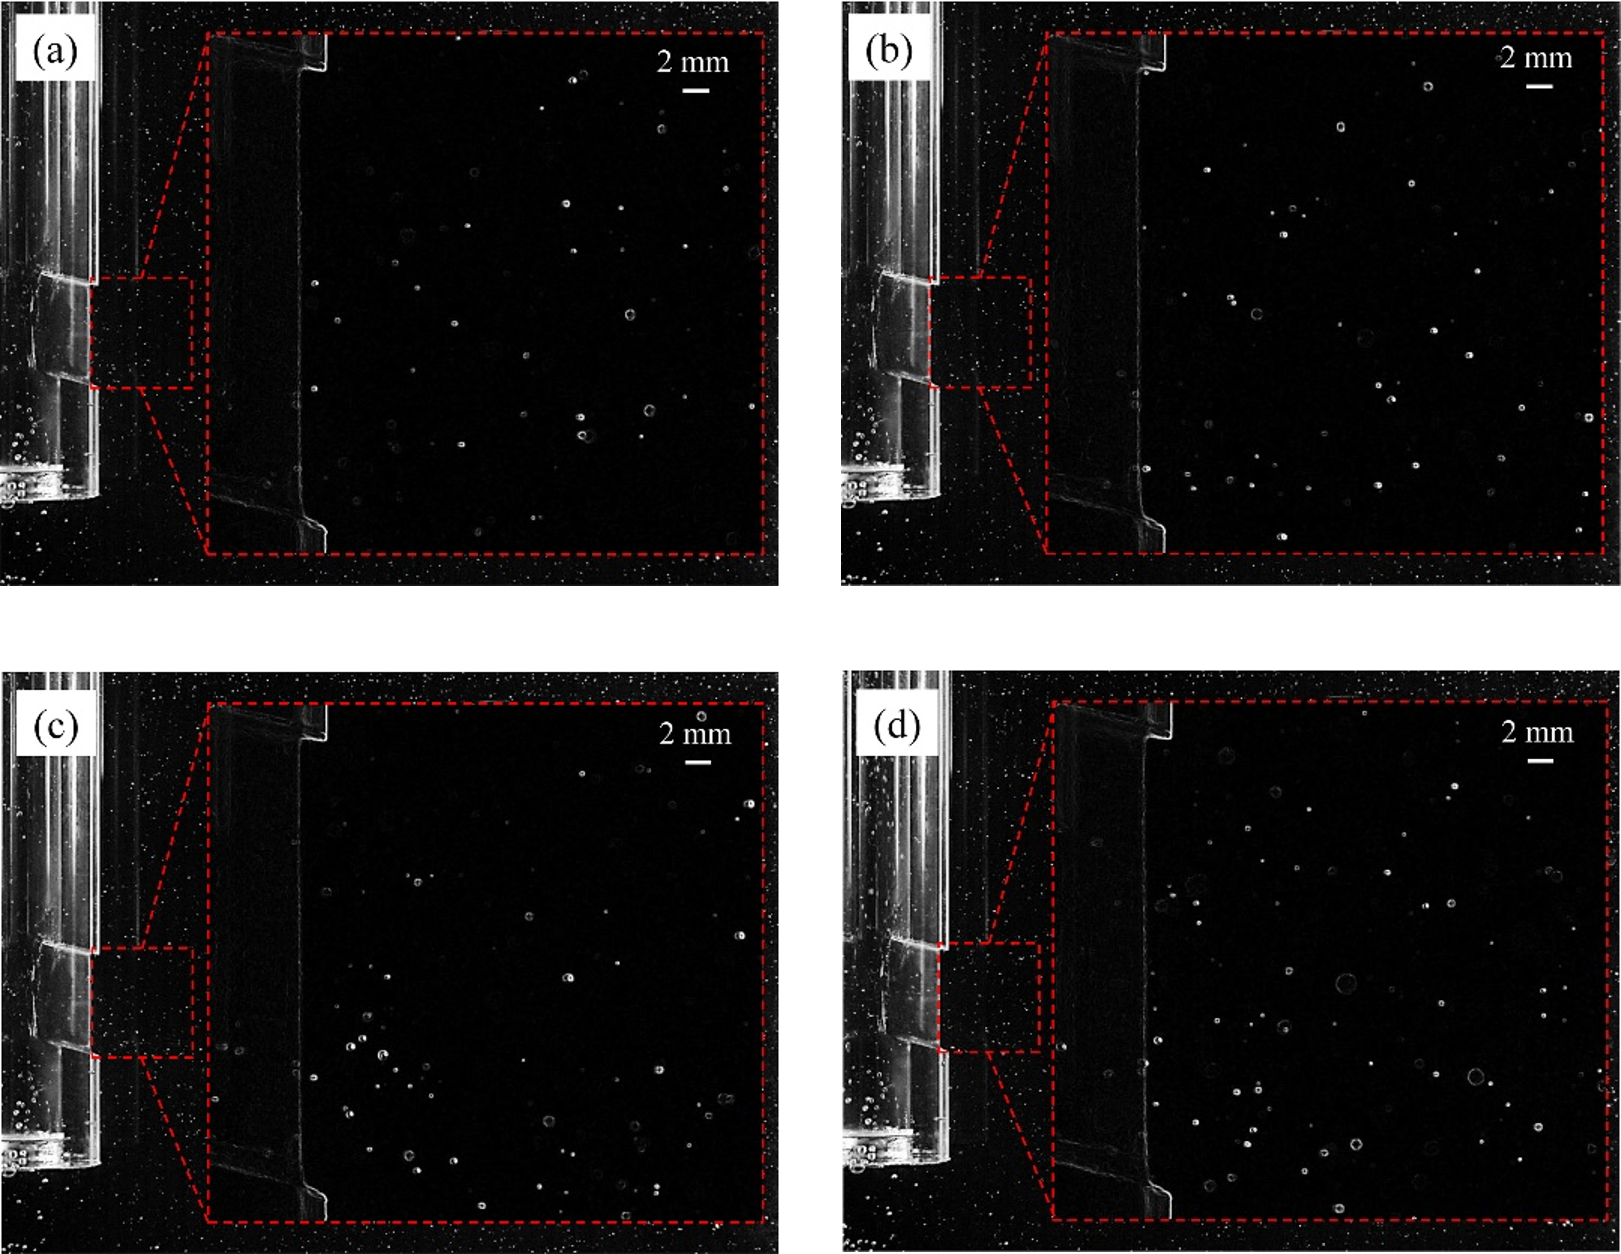
\includegraphics[width=1.0\textwidth]{Fig3-2.png}
    \bicaption{\boldmath 不同吹氩量下结晶器水模型内气泡形貌:(a)2 L·min$^{-1}$;(b)4 L·min$^{-1}$;(c)6 L·min$^{-1}$;(d)8 L·min$^{-1}$}
    {Bubble morphology in mold at different argon flow rates from water model experiment: (a) 2 L·min$^{-1}$; (b) 4 L·min$^{-1}$; (c) 6 L·min$^{-1}$; (d) 8 L·min$^{-1}$\\
    \textcolor{red}{(宋体、Times New Roman 5号字加粗,居中置于图的下方)}}
    \label{Fig3-1}
\end{figure}
\clearpage